 
%----------------------------------------------------------------------------------------
%	PACKAGES AND OTHER DOCUMENT CONFIGURATIONS
%----------------------------------------------------------------------------------------

\documentclass[fleqn,10pt]{SelfArx} 
\usepackage{caption}
\DeclareCaptionType{mycapequ}[][List of equations]

\captionsetup[mycapequ]{labelformat=empty}
 \usepackage{ragged2e}
 \usepackage{appendix}
\usepackage{float}
\usepackage{hyperref} 

%----------------------------------------------------------------------------------------
%	COLUMNS
%----------------------------------------------------------------------------------------

\setlength{\columnsep}{0.55cm} % Distance between the two columns of text
\setlength{\fboxrule}{0.75pt} % Width of the border around the abstract

%----------------------------------------------------------------------------------------
%	COLORS
%----------------------------------------------------------------------------------------

\definecolor{color1}{RGB}{0,0,90} % Color of the article title and sections
\definecolor{color2}{RGB}{0,20,20} % Color of the boxes behind the abstract and headings

%----------------------------------------------------------------------------------------
%	HYPERLINKS
%----------------------------------------------------------------------------------------



\hypersetup{hidelinks,colorlinks,breaklinks=true,urlcolor=color2,citecolor=color1,linkcolor=color1,bookmarksopen=false,pdftitle={Title},pdfauthor={Author}}


%----------------------------------------------------------------------------------------
%	ARTICLE INFORMATION
%----------------------------------------------------------------------------------------

\JournalInfo{Équations de réaction diffusion, 2018} 
\Archive{} 

\PaperTitle{La masse d'un mammouth : \\
étude d'un modèle convectif
} 
\Authors{Marine Djaffardjy\textsuperscript, Théophile Moreal de Brevans, Émilie Mathian } % Authors

\Keywords{Convection--- Schéma de Lax --- Règle de Cope --- Cladogenèse} %
\newcommand{\keywordname}{Keywords} 
%----------------------------------------------------------------------------------------
%	ABSTRACT
%----------------------------------------------------------------------------------------

\Abstract{\L'évolution de la masse des espèces animales au cours des ères géologiques est un processus complexe dépendant de nombreux facteurs biologiques et écologiques. Il a pourtant pu être mathématiquement modélisé. Les modèles sont fondés sur le postulat de Cope selon lequel la taille des espèces tend à augmenter au cours des générations. Cette règle, considérée comme universelle, s'applique à de nombreux clades (mammifères, oiseaux, ...). Elle permet d'expliquer l'allure générale de la distribution des masses. Modéliser cette distribution asymétrique grâce à à un terme convectif sera l'un des objectifs de notre étude. Nous tenterons aussi d'observer l'influence de la règle de Cope. % Développer les autres objectifs
~}
% Rmq irritante Les poissons ne forment pas un clade mais le mathématicien ne considère pas cette information comme cruciale ! :( 
%----------------------------------------------------------------------------------------

\begin{document}

\flushbottom % Makes all text pages the same height

\maketitle % Print the title and abstract box

\thispagestyle{empty} % Removes page numbering from the first page

%----------------------------------------------------------------------------------------
%	ARTICLE CONTENTS
%----------------------------------------------------------------------------------------

\section*{Introduction} % The \section*{} command stops section numbering

\subsection*{Fondamentaux biologiques}
La règle de Cope date de 1887 \cite{stanley1973explanation}. Suite à l'observation de fossiles, il fait le postulat de l'augmentation de la taille des espèces au cours des générations. Bien que cette règle générale soit controversée, les jeux de données actuels semblent la confirmer. L'une des principales critiques est à l'absence de prise en compte des liens phylogénétiques \cite{lovegrove2013evolution}. En effet, les modèles présument de l’indépendance des données (absence de liens de parenté), en raison de données phylogénétiques peu fiables. 
\\Le gain de taille prévu par la règle de Cope constitue un avantage sélectif. Biologiquement l'augmentation de la taille améliore la thermorégulation, l'endurance,  la compétition  inter-spécifique, ou encore l'accès aux ressources (augmentation de la gamme d'aliments disponibles) \cite{stanley1973explanation}. Un exemple d'adaptation de la taille des espèces face aux changements climatiques a été expliqué pour la période éocénique. Les températures ont fortement augmenté au début de l'éocène et ont induit la disparition des forêts pour laisser place à de vastes plaines. Ces nouvelles niches écologiques ont impliqué l'augmentation de la taille des membres des herbivores contraints par la prédation. De plus le passage à une alimentation essentiellement constituée de cellulose est mieux adaptée aux métabolisme des herbivores de grande taille. Le gain de taille des herbivores implique l'augmentation de celle des prédateurs qui doivent exploiter les proies de toutes tailles, restreignant de ce fait la taille de leurs proies \cite{lovegrove2013evolution}. Si la règle de Cope implique une augmentation générale de la taille des animaux, celle-ci n'interdit pas des phases de diminution, bien que plus rares. Toutefois, il a déjà été démontré que la taille des animaux  ne pouvait décroître en-dessous de certaines limites en raison de contraintes physiologiques et thermiques. Ceci permet d'imposer une limite inférieure à notre modèle. La distribution de la masse des espèces suit une forme canonique où la classe modale se situe autour de 40g et où les espèces de petite taille ou de grande taille sont non seulement peu communes mais ont également une répartition asymétrique. Ainsi le Mammouth Impérial aurait eu une masse $10^7$g alors que le plus petit mammifère, la musaraigne pygmée, pèse $1.8$g. Cette asymétrie autorise une limite supérieure peu contraignante. Enfin, le mécanisme crucial soutenant le modèle est que l'augmentation de taille accroît le risque d'extinction \cite{clauset2008many}. % à expliquer  
\section*{Modèle et paramètres}
\subsection*{Modèle de Aaron Clauset}
Aaron Clauset \cite{clauset2008many}\cite{clauset2013large} est l'auteur de plusieurs études s'intéressant aux modèles de diffusion de la masse modélisée par l'équation suivante :
\begin{equation}
\frac{\partial f}{\partial t}+\nu \frac{\partial f}{\partial x} = D \frac{\partial^2 f}{\partial x^2} + (1-A-Bx)f 
\label{eq1}
\end{equation}
$f(x,t)$ représente le nombre d'espèces ayant une masse équivalent à $x=\ln(M)$ au temps t. Le paramètre $\nu = <\ln\lambda>$ est le biais de masse entre l'ancêtre et son descendant, $D$ le coefficient de diffusion équivaut à $D=<(\ln\lambda)^2>$. Le paramètre $\lambda$ est une variable aléatoire tirée d'une loi log-normale de paramètre $\nu$, ou une constante selon les simulations.  $D$ traduit pour chaque événement de spéciation un la masse peut être biaisée vers la gauche ou vers la droite. 

 D'après la règle de Cope $\ln\lambda >0$. Enfin $A-Bx$ traduit la probabilité d'extinction d'une espèce, corrélée au logarithme de la masse par le coefficient $B>0$.\\
\subsection*{Conditions initiales et conditions aux bords}
Nous allons étudier cette équations avec deux types de conditions aux bords. Premièrement avec les conditions de Dirichlet-Neumann. Nous faisions ainsi les hypothèses sont que le poids minimal 2g ,compatible avec les vie, ne peut être franchi et qu'il peut exister un flux au bord droit. Secondement nous étudierons le modèle avec les conditions de Dirichlet-Dirichlet, ce qui nous permet à nouveau de limiter la diffusion en deçà de 2g mais également de représenter l'absence de flux au niveau du bord droit. Sous cette hypothèse nous modélisons l'extinction des espèces ayant une masse en dessus d'une certaine limite fixée à $10^7g$. Celle-ci peut être atteignable d'après les conditions biologiques déterminées mais reste néanmoins peu probable.  

\subsection*{Simplification du modèle}
Retirons le terme de convection pour l'analyse mathématique l'équation \ref{eq1} s'écrit telle que :
\begin{align}
\frac{\partial f}{\partial t}= D \frac{\partial^2 f}{\partial x^2} + (1-A-Bx)f \nonumber\\
\frac{\partial f}{\partial t}= D \Delta_xf+ (1-A-Bx)f \label{eq2}
\end{align}
\subsubsection*{Fonctions propres :}
Nous cherchons à présent les fonctions propres, notées $\omega(x)$, associées au deux types de conditions.
Rappelons que les fonctions propres ($\omega(x)$), avec $x\in [0,M]$ doivent vérifier :
\begin{enumerate}
\item $\omega(x)$ est au moins deux fois dérivable,
\item Il existe $\lambda \in \mathbb{R}$ tel que $\omega(x)^{\prime \prime}=\lambda\omega(x)$
\item $\omega(x) \equiv 0$ \label{cond2}
\end{enumerate}
On cherche donc les solutions telles que $\omega(x)^{\prime \prime}=\lambda\omega(x)$ les solutions sont donc de la forme $\omega(x) = e^{rx}$ ainsi $\omega(x)^{\prime}=re^{rx}$, et $\omega(x)^{\prime \prime}=r^2e^{rx}$ d'où $r^2e^{rx}= \lambda e^{rx}$. On obtient $r^2=\lambda$.\\
\underline{Pour les conditions de Dirichlet-Neumann :}\\
D'après ces conditions aux bords on a par définition $\omega(0)=0$ et $\omega(M)^\prime =0$\\
\underline{Cas 1  $\lambda > 0$ :}\\
On obtient deux racines réelles $r_1 = \sqrt{\lambda}$ et  $r_2 = -\sqrt{\lambda}$, et deux solutions $\omega_1(x)= e^{r_1x}$ et $\omega_2(x)= e^{r_2x}$. Par combinaison de ces deux solutions on a :
\begin{align*}
\omega(x) =C_1+ e^{r_1x}+ C_2e^{-r_1x} \\
\omega^\prime(x) = r_1(C_1 + e^{r_1x} - C_2e^{-r_1x})
\end{align*}

Or d'après la condition de Dirichlet on a :
$\omega(x)=0 \Rightarrow C_1 + C_2=0 $ $ \Rightarrow C_1 =C_2$. On peut réécrire la fonction $\omega(x)$ telle que $\omega(x)= C_1(e^{r_1x}- e^{r_2x })$.\\
D'après la condition de Neumann on a :
$$\omega(M)^\prime = 0  \Rightarrow r_1C_1(e^{r_1M}+e^{r_2M}) =0 $$

On a alors deux solutions possibles :
\[
\left\{
\begin{array}{r c l}
C_1 =0\\
e^{r_1M} + e^{r_2M} =0
\end{array}
\right.
\]
Or comme $M>0$ ceci implique que $e^{r_1M} + e^{r_2M} >0$. Donc on aurait $C_1=0$ et $C_2 =0$, ce qui est impossible dans le cadre de la troisième condition.\\
\underline{Cas 2  $\lambda = 0$ :}\\
Si $\lambda = 0$ alors $r=0$, on a alors $\omega(x)^{''}=0\Rightarrow \omega(x)^{'}=0$et $\omega(x)=C_1x+C_2 $.

D'après Dirichlet on a $\omega(0)=0$  donc $C_2=0$. Notre fonction propre peut alors être écrite telle que $\omega(x)=C_1x\Rightarrow \omega(x)\prime=C_1$, d'après les conditions de Neumann on a :\\
$\omega(M)'=0 $ et donc $C_1=0$ ce qui est impossible en vertu de la condition 3.

\underline{Cas 3  $\lambda < 0$ :}\\
On obtient deux racines complexes telles que : \\
$r_1 = i\sqrt{|\lambda|} $ et $r_2 = -i\sqrt{|\lambda|}$ de la forme $r = \alpha + i\beta$ et deux solutions possibles $\omega_1(x)= e^{i\sqrt{|\lambda|x}}$ et $\omega_2(x)= e^{-i\sqrt{|\lambda|x}}$ .\\
Les solutions sont alors données par :
$$ \omega(x) = e^{\alpha x}(C_1 \cos(\beta x) + C_2 \sin(\beta x) ) $$
où $\alpha = 0$ et $\beta = \sqrt{|\lambda|}$ donc $$\omega(x) =C_1 \cos(\sqrt{|\lambda|} x) + C_2 \sin(\sqrt{|\lambda|} x)$$ \\
et $\omega^\prime(x) =\sqrt{|\lambda|}(C_1 \sin(\sqrt{|\lambda|} x) + C_2 \cos(\sqrt{|\lambda|} x)) $. \\
D'après les conditions de Dirichlet on a :
$$ \omega(0)=0 \Rightarrow \sqrt{|\lambda|}(C_1 \sin(0) + C_2 \cos(0)) =0$$
donc $C_1=0$, on peut réécrire $\omega(x)$ telle que : 
$$\omega(x) = C_2 sin(\sqrt{|\lambda|}x)\Rightarrow \omega(x)' = \sqrt{|\lambda|}C_2cos(\sqrt{|\lambda|}x)$$
Or d'après les conditions de Neumann $\omega(M)'=0$ donc \\
$\sqrt{|\lambda|}C_2cos(\sqrt{|\lambda|}M=0)$

On a deux solutions sont possibles :
\[
\left\{
\begin{array}{r c l}
C_2 =0\\
\cos(\sqrt{|\lambda |}M  =0
\end{array}
\right.
\]

Pour respecter la condition 3 la seule solution possible est $\cos(\sqrt{|\lambda |}M =0 \Rightarrow \sqrt{|\lambda |}M = \frac{k\pi}{2} $. On déduit que les valeurs propres sont de la forme $\lambda_k =- (\frac{-k\pi}{2M})^2$ et les fonctions propres sont telles que $\omega_k(x)=C_2 sin (\frac{-k\pi}{M}x)$, ce qui peut être généralisé par $\omega_k(x)= sin (\frac{-k\pi}{M}x)$.\\

\underline{Pour les conditions de Dirichlet-Dirichlet :}

D'après ces conditions aux bords on a par définition $\omega(0)=0$ et $\omega(M)\prime =0$\\
\underline{Cas 1  $\lambda > 0$ :}\\
On obtient deux racines réelles $r_1 = \sqrt{\lambda}$ et  $r_2 = -\sqrt{\lambda}$, et deux solutions $\omega_1(x)= e^{r_1x}$ et $\omega_2(x)= e^{r_2x}$. Par combinaison de ces deux solutions on a :
\begin{align*}
\omega(x) =C_1+ e^{r_1x}+ C_2e^{-r_1x}\\
\omega^\prime(x) = r_1(C_1 + e^{r_1x} - C_2e^{-r_1x})
\end{align*}

Or d'après la condition de Dirichlet on a :
$$\omega(x)=0 \Rightarrow C_1 + C_2=0  \Rightarrow C_1 =C_2$$.
On peut réécrire la fonction $\omega(x)$ telle que $\omega(x)= C_1(e^{r_1x}- e^{r_2x })$.\\
D'après la seconde condition de Dirichlet on a :
$$\omega(M) = 0  \Rightarrow C_1(e^{r_1M}+e^{r_2M}) =0 $$

On a alors deux solutions possibles :
\[
\left\{
\begin{array}{r c l}
C_1 =0\\
e^{r_1M} + e^{r_2M} =0
\end{array}
\right.
\]
Or $r_1M = ln(M)=0$ impliquerait que $\omega(x) \equiv 0$ ce qui est impossible en raison de la troisième condition.

\underline{Cas 2  $\lambda = 0$ :}\\
Si $\lambda = 0$ alors $r=0$, on a alors $\omega(x)^{''}=0\Rightarrow \omega(x)^{'}=0$ et $\omega(x)=C_1x+C_2 $.

D'après Dirichlet on a $\omega(0)=0$  donc $C_2=0$. La fonction $\omega(x)$ peut alors être écrite telle que $\omega(x)=C_1x$. Or d'après la seconde condition de Dirichlet $\omega(M)= C_1M = 0 \Rightarrow C_1=0$. En raison de la condition 3 cette solution est impossible.

\underline{Cas 3 : $\lambda < 0$ :}\\
On obtient deux racines complexes telles que : \\
$r_1 = i\sqrt{|\lambda|} $ et $r_2 = -i\sqrt{|\lambda|}$ de la forme $r = \alpha + i\beta$  .\\
Les solutions sont alors données par :
$$ \omega(x) = e^{\alpha x}(C_1 \cos(\beta x) + C_2 \sin(\beta x) ) $$
où $\alpha = 0$ et $\beta = \sqrt{|\lambda|}$ donc $$\omega(x) =C_1 \cos(\sqrt{|\lambda|} x) + C_2 \sin(\sqrt{|\lambda|} x)$$ \\
et $\omega^\prime(x) =\sqrt{|\lambda|}(C_1 \sin(\sqrt{|\lambda|} x) + C_2 \cos(\sqrt{|\lambda|} x)) $. \\
D'après les conditions de Dirichlet on a :
$$ \omega(0)=0 \Rightarrow \sqrt{|\lambda|}(C_1 \sin(0) + C_2 \cos(0)) =0$$
donc $C_1=0$, on peut réécrire $\omega(x)$ telle que :
$$\omega(x) = C_2 sin(\sqrt{|\lambda|}x)$$

Or d'après la seconde condition de Dirichlet $\omega(M)=0$ donc : 
$$\sqrt{|\lambda|}C_2sin(\sqrt{|\lambda|}M=0)$$

On a deux solutions possibles :
\[
\left\{
\begin{array}{r c l}
C_2 =0\\
\sin(\sqrt{|\lambda |}M  =0
\end{array}
\right.
\]

Pour respecter la condition 3 la seule solution possible est $\sin(\sqrt{|\lambda |}M =0 \Rightarrow \sqrt{|\lambda |}M = \frac{k\pi}{2} $. On déduit que les valeurs propres sont de la forme $\lambda_k =- (\frac{-k\pi}{M})^2$ avec $k\in \mathbb{N^*}$ et les fonctions propres sont telles que $\omega_k(x)=C_2 sin (\frac{k\pi}{M})$, ce qui peut être généralisé par $\omega_k(x)= sin (\frac{k\pi}{M})$.\\

\subsubsection*{Estimation des paramètres :} 
Reprenons l’estimation statistiques des paramètres du modèle établit sur un jeu de données répertoriant 4022 espèces de mammifères fossiles \cite{clauset2008evolution} :
\begin{itemize}
\item $x_{min}$ = 2g
\item $x_{max}= 10^7$g
\item $A = 0.221$
\item $B = 0.4064 $
\item $D = 0.508 $
\item $\nu = 0.109 $ 
\end{itemize}
Rappelons par ailleurs que le modèle estime la distribution du logarithme de la masse.
\subsubsection*{Caractérisation des équilibres :} 
% Sans conviction
Notons $f^*$ les équilibres de l'équation \ref{eq2} rappelons que ceux-ci vérifient :
$$\frac{\partial f^*}{\partial t} =0 \quad \text{et} \quad \Delta xf^*=0 $$
Alors on a $(1-A-Bx)f^*=0$ notons $g(f,x)$ la fonction telle que : 
$$g(f,x) =(1-A-Bx)f$$
Nous avons donc deux équilibres notés $f^*_0=0$ et $x^*_0=  \frac{1-A}{B}$. 
\subsubsection*{Étude de la stabilité :} 
\underline{Au point d'équilibre $f^*_0$ } : \\
$$\frac{\partial g}{\partial f} = (1-A-Bx) \rightarrow g(f^*_0 , x)^\prime = (1-A-Bx)$$
D'après nos conditions  $\lambda_k =-(\frac{k\pi}{2M})^2 $ et l'estimation des paramètres nous obtenons :
\begin{align*}
g(f^*_0 , x)^\prime + D \lambda_k = (1-A-Bx) - D(\frac{\pi}{M}) ^2k^2\\
= 1 - 0.2221 - 0.4064 x - 0.508(\frac{\pi}{ln(10^7)})^2k^2
% M = x_max ?
% A recalculer avec les nouveaux paramètres
\end{align*}
Cet équilibre est localement asymptotiquement stable (LAS) si $g(f^*_0 , x)^\prime + D \lambda_k <0 $ donc si $k \in [-\sqrt{\frac{A-1+Bx}{-D(\pi /M)^2}},\sqrt{\frac{A-1+Bx}{-D(\pi /M)^2} ]}$. Les solutions de cette inéquation existent si $x>6.8$g, soit lorsque x tend vers l'infini.\\
D'après cette caractérisation nous pouvons affirmer qu'il existe un moment où la répartition de la masse sera à l'équilibre, et donc qu'il existe une condition optimale de stabilité des espèces en terme de masse.\\
\underline{Au point d'équilibre $x^*_0$ } : \\
$$\frac{\partial g}{\partial x} = Bf \rightarrow g(f , x^*_0)^\prime = Bf$$
De même cet équilibre est LAS si $g(f , x^*_0)^\prime + D \lambda_k <0 $. Or par hypothèse $f(x,t) >0$ et comme $D\lambda_k$ <0, cette équilibre sera instable quelle que soit k. \\
L'interprétation de cette équilibre reste relativement, en effet il implique qu'un ensemble d'espèce de mammifères d'une masse proche de 2g risquent de s'éteindre ou d'augmenter en masse.


\section*{Implémentation numérique}
Afin d'observer l'influence du terme de convection, nous proposons d'implémenter deux modèles un premier sans ce terme de convection et un second prenant en compte ce dernier. Nous étudierons le problème par deux approches numériques, dans un premier temps avec un modèle continu dans le temps, puis par une modélisation individu centré.
% Schéma sans convection partie théophile

\subsection*{Schéma numérique continu}
%%% SUite partie Théophile
\subsubsection*{Schéma sans convection }
La simulation effectuée avec ce modèle donne à voir une distribution gaussienne dans les premiers temps. Puis, au bout d'un temps suffisamment grand la distribution perd ce caractère gaussien en s'étalant sur la gamme de masses autorisée par le modèle (fig. 1). On perd donc la valeur modale de 40g observée dans les données au profit des espèces de masse minimale. L'intervalle des densités est également très réduit.

\begin{figure}[H]
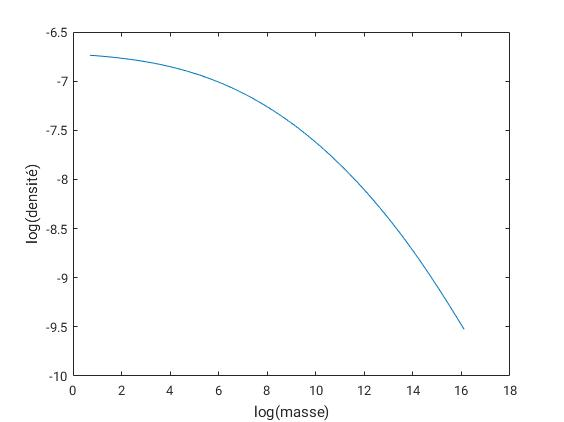
\includegraphics[scale=0.4]{courbe_neuneu_sans.jpg}
\caption{Distribution de la masse des espèces d'après le modèle sans convection en échelle log(densité)=f(log(masse))}
\end{figure}

Précisons que la figure 1 est obtenue avec des conditions de Neumann imposées aux bords. Le modèle serait sûrement plus proche des données si on imposait une condition de Dirichlet à gauche pour tenir compte de l'impossibilité physiologique pour un mammifère de peser moins de 2g. Si on fixe la valeur 2g à 0, on obtient la courbe suivante (fig. 2) après un temps de simulation grand.

\begin{figure}[H]
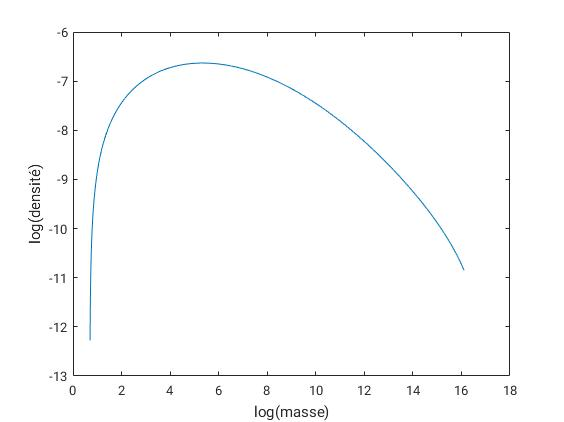
\includegraphics[scale=0.4]{courbe_dirneu_sans.jpg}
\caption{Distribution de la masse des espèces d'après le modèle sans convection en échelle log(densité)=f(log(masse))}
\end{figure}

L'ajout du terme de convection a présenté certaines difficultés algorithmiques qui nous ont conduit à utiliser la méthode de Lax-Friedrichs.
\subsubsection*{Schéma avec convection}
Afin de simplifier l'implémentation numérique de l'équation (\ref{eq1}), nous proposons de scinder cette équation en une somme de plusieurs termes. Nous avons choisi le schéma de Lax-Friedrichs pour calculer le terme de convection $\nu \frac{\partial f}{\partial x}$, la méthode de Crank Nicolson pour la diffusion et un schéma explicite pour le terme de réaction. Écrivons à présent la méthode numérique, le pas de temps est noté $n$ et le pas d'espace $j$, enfin la fonction $f(x,t)$ discrétisée est notée $U$. \\
\underline{Schéma de Lax-Friedrichs - convection :}
\begin{align*}
\frac{\partial U}{\partial t}+\nu \frac{\partial U}{\partial x} &= \nu \frac{U_{j+1} ^n - U_{j-1}^n}{2\Delta x}  + \frac{ U_j^{n+1} - \frac{1}{2}U_{j+1}^n + U_{j-1}^n}{\Delta t}
\end{align*}
\underline{Schéma de Crank Nicholson - Diffusion:}
\begin{align*}
\frac{\partial U}{\partial t} &= D\frac{\partial^2U}{\partial x^2}\\
\frac{U_j^{n+1} - U_j^n}{\Delta t} &=D\frac{(U_{j+1}^{n+1} -2U_{j}^{n+1} }{\Delta x)^2}\\
&- \frac{U_{j-1}^{n+1}) + U_{j+1}^{n} -2U_{j}^{n} + U_{j-}^{n})}{2(\Delta x)^2}
\end{align*}
\underline{Schéma explicite - Réaction}
\begin{align*}
 \frac{\partial U}{\partial t} &= f(t, U) \\
 U_{j+1}^n &= U_{j}^n + \Delta t (1-A-Bx) U_j^n
\end{align*}
Finalement en isolant le terme $U_j^{n+1}$ nous obtenons un schéma de forme générale :
\begin{align*}
\frac{U_j^{n+1}}{\Delta t} = - \frac{1/2}{\Delta t}(-U_{j+1}^n +U_{j-1}^n )+ \\ 
\frac{D}{2}\frac{L_0^{n+1}+L0^n}{\Delta x^2}- \nu \frac{U_{j+1} ^n - U_{j-1}^n}{2\Delta x} +(1-A-Bx) U_j^n
\end{align*}

avec L0 une matrice trigonale telle que : 
$$
% Faux à changer
L0 = \begin{pmatrix}
    -2 & 1    & \cdots & 0 \\ 
    \vdots & 1 & -2 & 1 & \vdots \\ 
    0      & \cdots & 1 & -2
\end{pmatrix}
$$
Afin de modéliser les deux types de conditions aux bords nous n'omettrons pas de modifier les coefficient $L0(1,1)$ et $L0(J,J)$
\newline
\subsubsection*{Résultats et interprétation}
Pour modéliser l'évolution des espèces de mammifères durant le crétacé nous avons avec convection nous avons conservé les paramètres cités ci-dessus pour A, B et $\nu$. Nous avons choisi un poids minimal de 2g étant la condition au bord Dirichlet et un poids maximal de $10^7$g représentant une condition de Dirichlet ou de Neumann selon la simulation. L'espace a été discrétisé avec un pas de 0.01. Enfin nous avons effectué une simulation sur 60 millions d'années période recouvrant les données \cite{clauset2008evolution}.

\begin{figure}[htb]
\centering
  \begin{tabular}{c}
    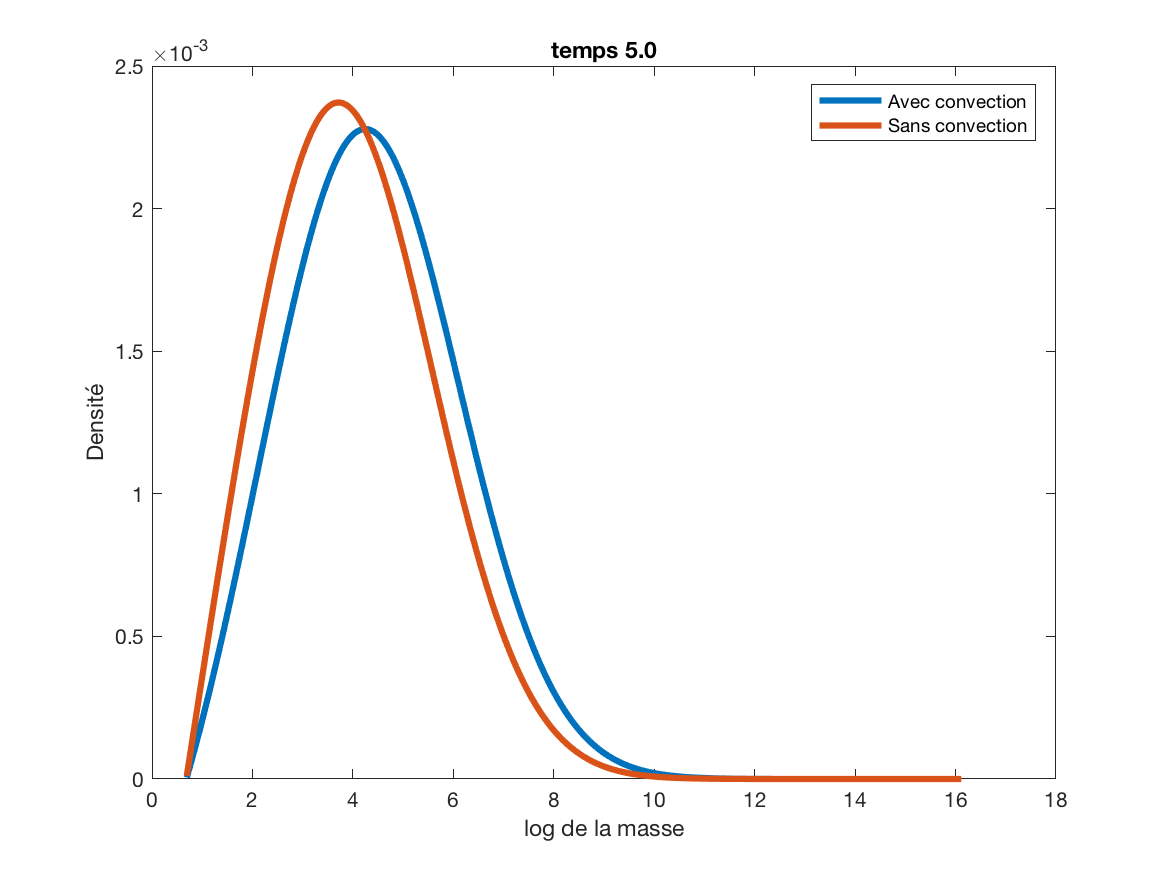
\includegraphics[width=.23\textwidth]{FIG_SC_AC5_0.png} \\
    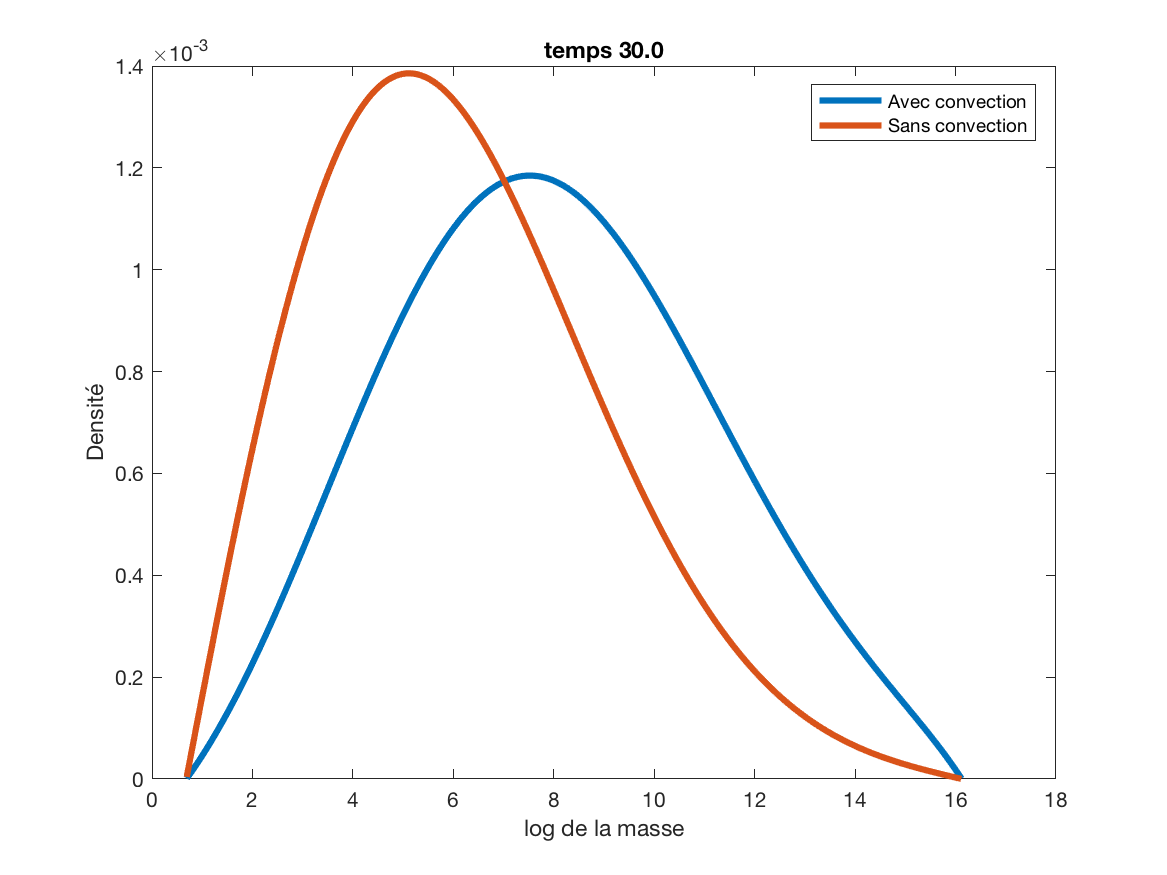
\includegraphics[width=.23\textwidth]{FIG_SC_AC30_0.png} \\
    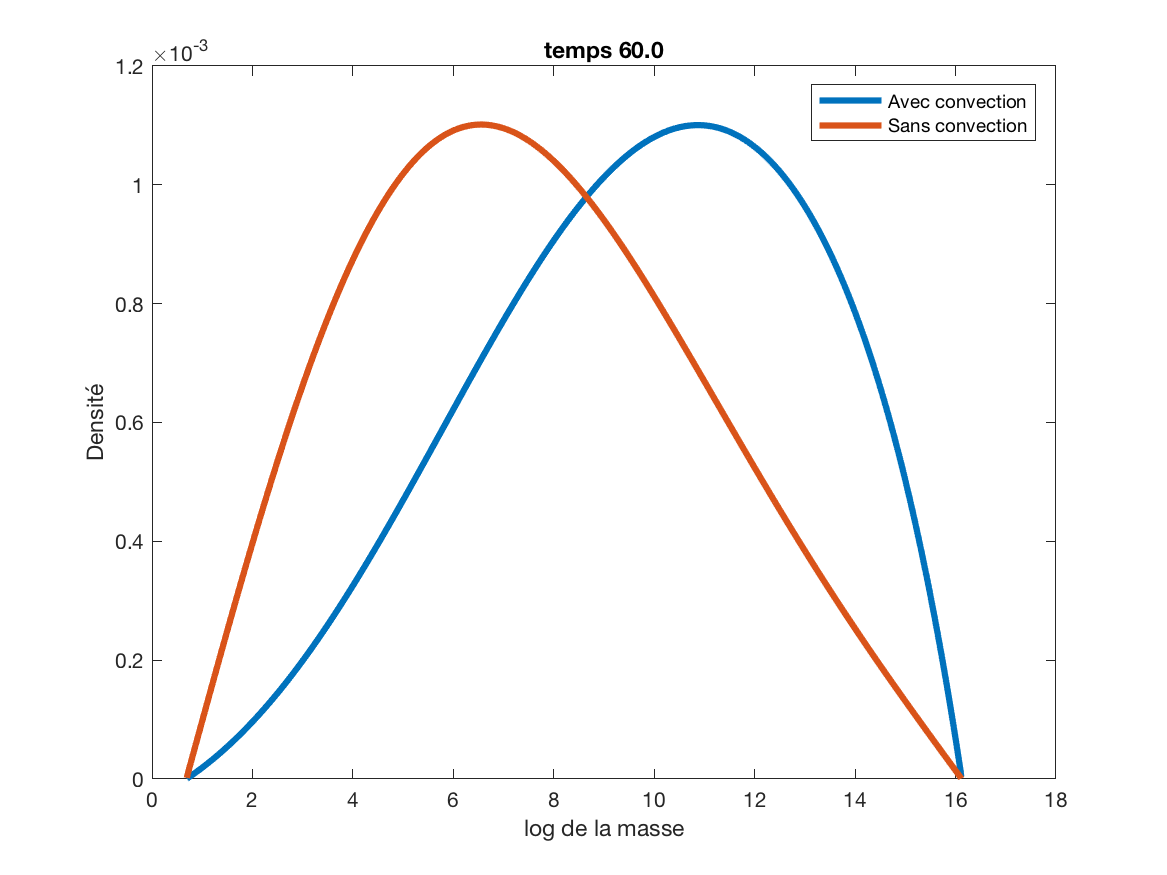
\includegraphics[width=.23\textwidth]{FIG_SC_AC60_0.png} \\ 
  \end{tabular}
  \caption{Densité des poids en fonction de log de la masse sans convection (rouge) avec convection (bleu) avec les conditions de Dirichlet-Dirichlet : Graphique 1) t=5M années , Graphique 2) t=30M années,  Graphique 3) t=60M années }
 \end{figure}


\begin{figure}[h]
\centering
  \begin{tabular}{c}
    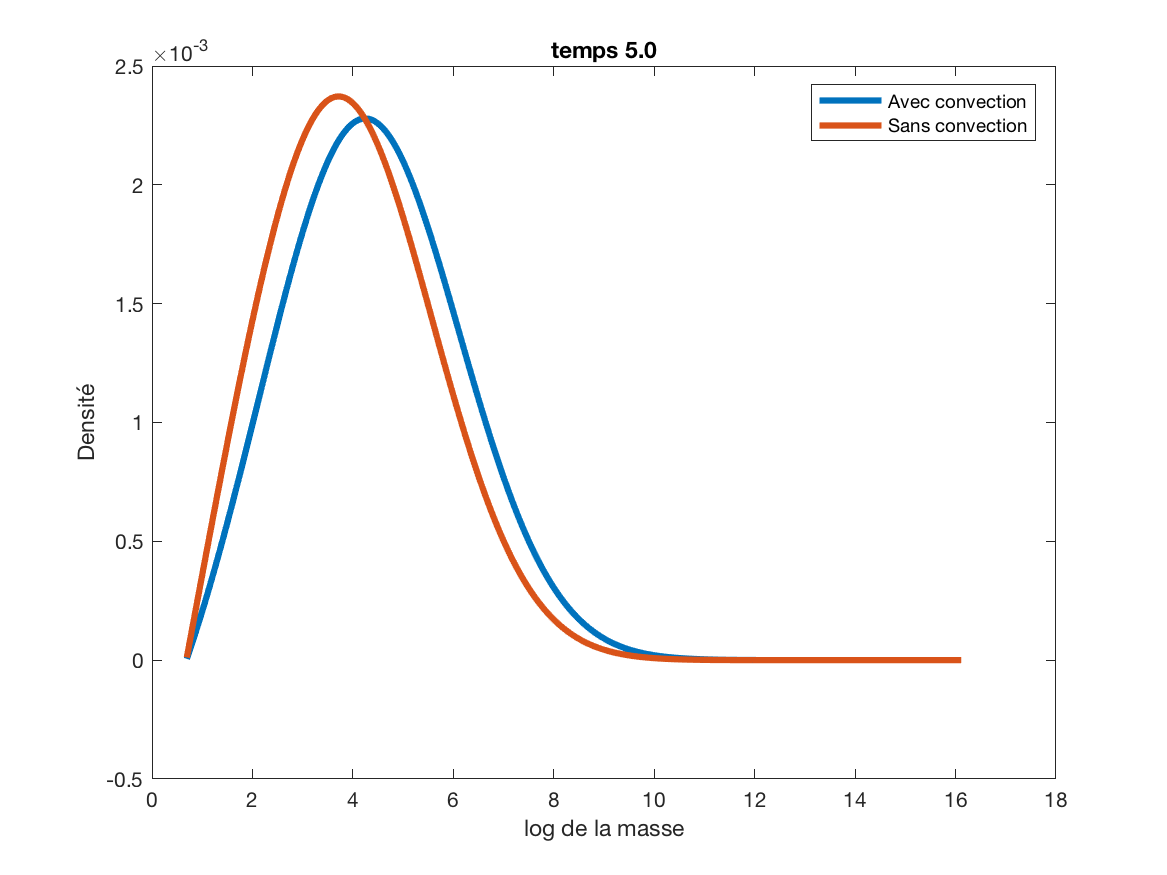
\includegraphics[width=.23\textwidth]{FIG_SC_AC_DN5_0.png} \\
    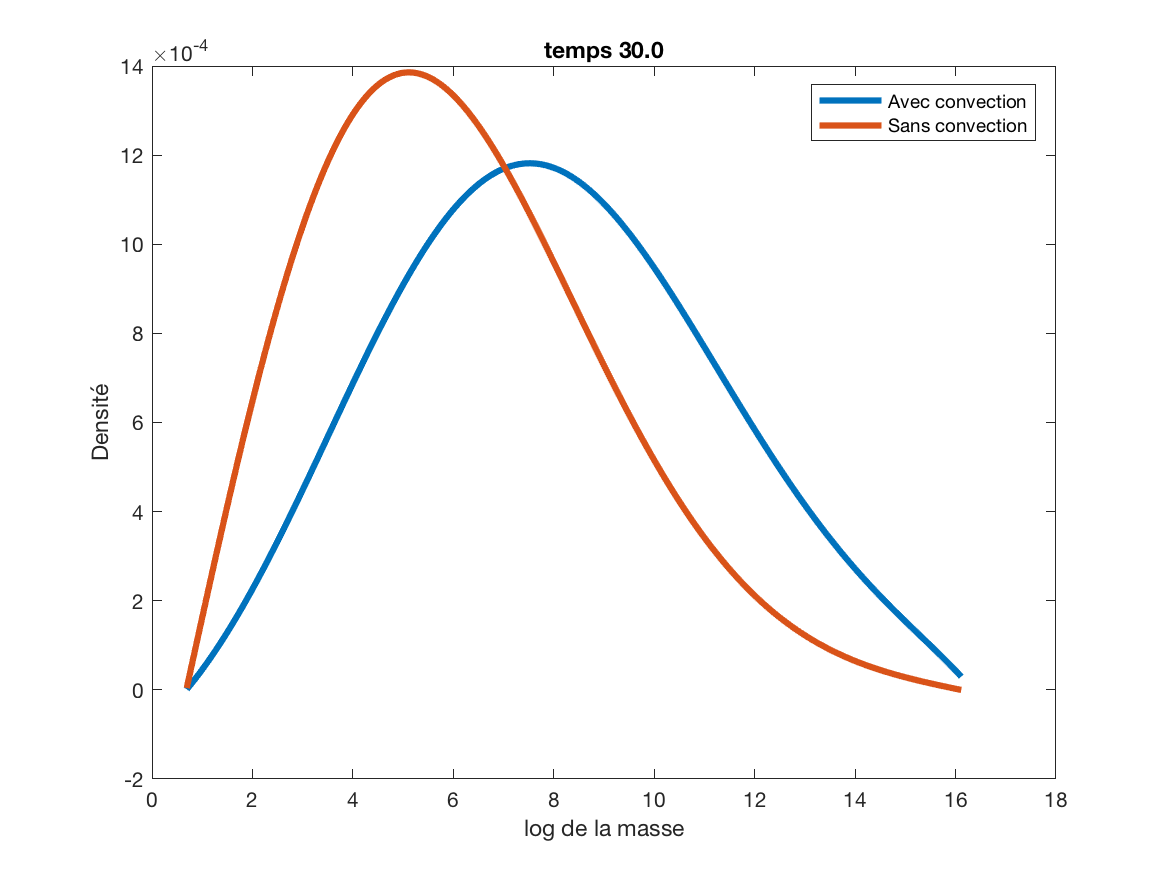
\includegraphics[width=.23\textwidth]{FIG_SC_AC_DN30_0.png} \\
    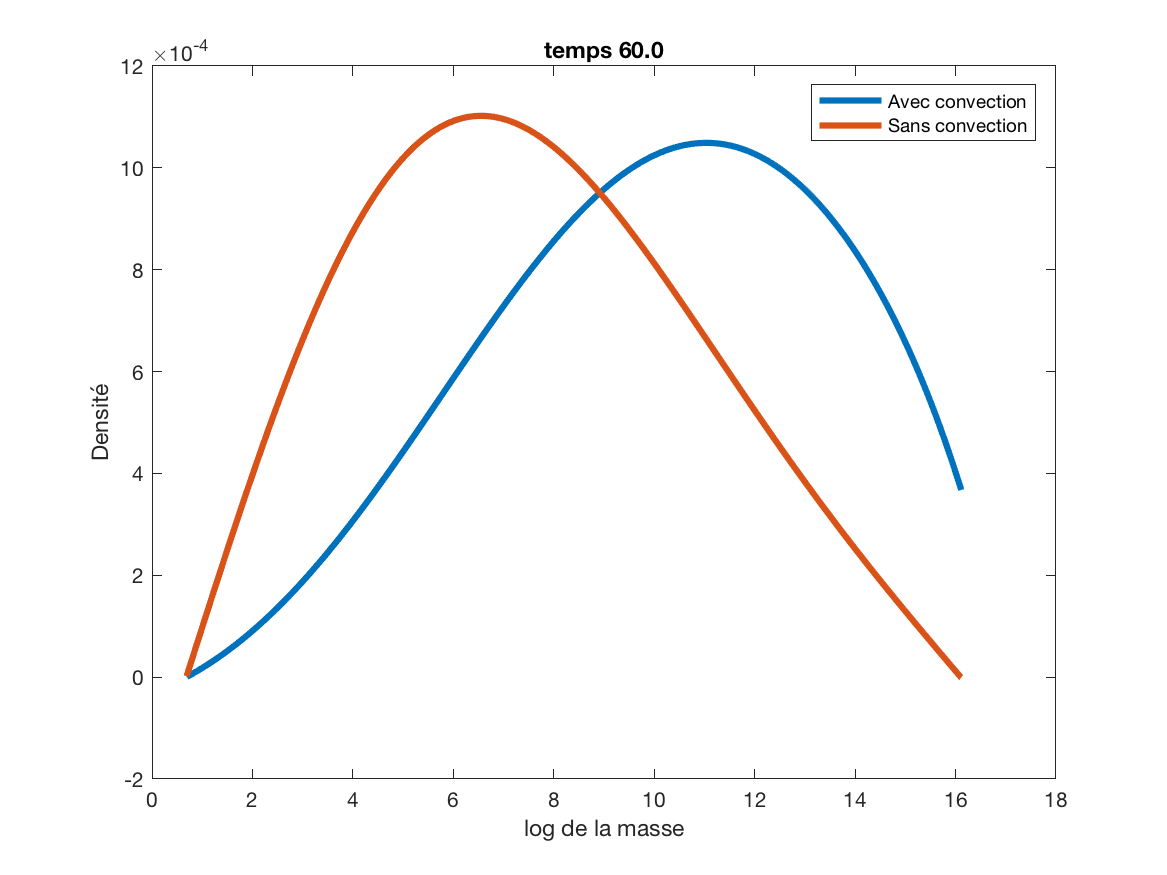
\includegraphics[width=.23\textwidth]{FIG_SC_AC_DN60_0.png} \\ 
  \end{tabular}
  \caption{Densité des poids en fonction de log de la masse sans convection (rouge) avec convection (bleu) avec les conditions de Dirichlet-Neumann : Graphique 1) t=5M années , Graphique 2) t=30M années,  Graphique 3) t=60M années }
 \end{figure}

Au regard des résultats, le terme de convection permet de générer un biais sur la diffusion. Au lieu d'observer une simple dispersion non orientée de la masse au cours de la cladogenèse, l'ajout du terme de convection permet de modéliser la règle de Cope. En effet celle-ci permet d'introduire le fait que l'augmentation de la masse augmente la fitness des espèces. La masse permettrait ainsi une meilleure thermorégulation, ou encore de faciliter l'accès aux ressources. Or si la convection permet de représenter cet effet, pourrait-on imaginer  une augmentation de masse jusqu'à l'infini? Étant donné que les hypothèses physiologiques ne contraignent le modèle dans ce sens, nous avons choisi de fixer une condition au bord supérieur très supérieure à la masse espèces mammifères fossiles et actuelles connue avec un poids maximal de 100 tonnes. \\
Néanmoins les hypothèses sous-jacentes d'une modélisation avec une condition de Dirichlet ou de Neumann diffèrent. En effet la condition de Dirichlet implique qu'une espèce de masse supérieure à la plus volumineuse ne peut exister, tandis qu'une condition de Neumann implique qu'elle ne peut engendrer une espèces plus grande. Toutefois l'une des caractéristique du modèle est que la masse maximale fixée par la condition au bord droit n'est pas atteinte à la fin de la simulation, ce qui suggère une autre contrainte à la borne supérieure. Celle-ci peut être expliquée par la compromis entre le gain de fitness permis par une augmentation de la masse et l'augmentation du risque d'extinction corrélé avec la masse, qui est contrôlé par la constante B de l'équation.  \\





\subsection*{Schéma individu-centré}
Ce schéma prend en sorte la convection.
\\La convection est prise en compte sous forme d'un paramètre de "biais", que nous allons utiliser pour appliquer la règle de Cope : le biais est plus grand (et fonction de la masse) pour les petites masses, et uniforme et inférieur pour les plus grandes masses. "Petites masses" correspond aux masses inférieures à un paramètre qui est le logarithme de l'intercept de la taille. 
\\Ce paramètre, en particulier, sert à modéliser le premier "virage" qu'on observe sur la courbe de la répartition des masses (il y en a un deuxième vers les grandes masses). Ces valeurs semblent justifier la règle de Cope, qui fait l'hypothèse que plus des animaux sont petits, plus ils ont tendance à grandir lors de l'évolution.
\\On peut observer ce virage sur cette courbe :

\begin{figure}[H]
\centering
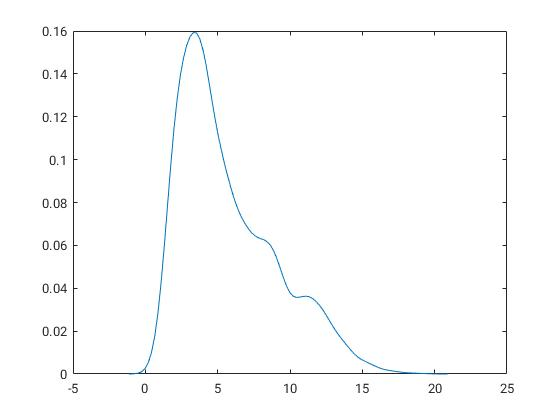
\includegraphics[width =5 cm]{empirique.jpg}
\caption{ Répartition empirique de la masse d'espèces mammifères du crétacé}
\end{figure}

Ce biais est pris en compte lors de l'étape de cladogénèse : en effet, à chaque tour, l'espèce (qui fait office d'individu dans le modèle), stocké sous forme de a masse moyenne des individus dans un vecteur, a une probabilité d'évoluer. Son évolution sera modélisée comme la disparition de l'espèce et l'apparition de deux autres espèces, différentes. Leurs masses dépendront de la masse de l'individu(espèce) mère. En effet, les masses des nouvelles espèces ne peuvent pas être trop éloignées de l'espèce mère.
\\Les espèces ont aussi, à chaque tour, une probabilité d'extinction, mais elle n'est pas fonction de la masse.
\\On a fait la simulation avec plusieurs paramètres : sans biais (donc sans paramètre de convection), avec un biais pour modéliser le premier virage, et avec un deuxième paramètre de biais pour tenter de modéliser le deuxième.

\begin{figure}[H]
\centering
    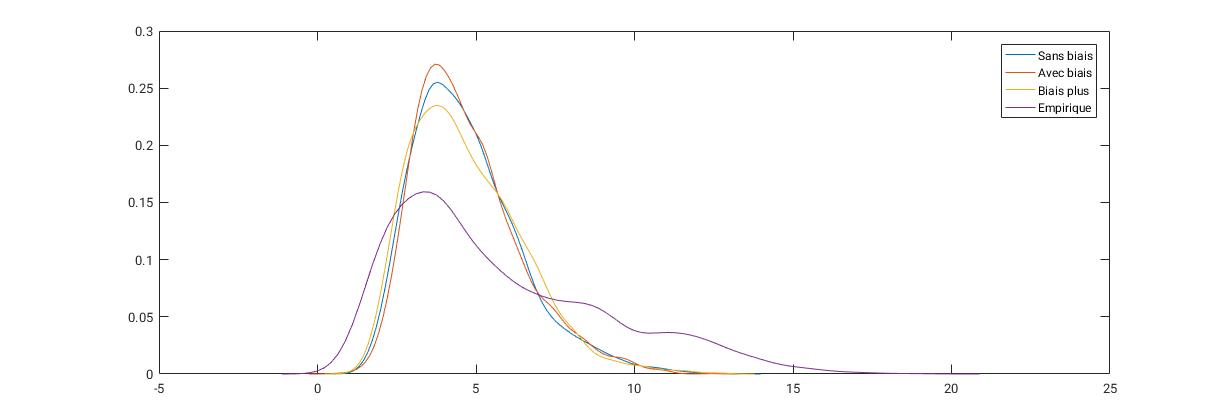
\includegraphics[width =0.5\textwidth]{comparaisongraphes.jpg}

\end{figure}

On peut voir que les différences entre les distributions des logarithmes des masses sont plus importants entre les modélisations qu'avec les données empiriques. Le paramètre de convection, notamment, ajoute une différence dans la répartition.
\\Le deuxième virage a été modélisé sur le même modèle que le premier : En utilisant un palier de la même forme, en choisissant un biais sur le même modèle... Mais il aurait pu être amélioré pour mieux coller à l'allure des données empiriques, même si c'est celui qui est le plus proche. On peut donc se pencher sur cette question et suggérer que la raison de ce virage n'a rien à voir avec la règle de Cope, mais à d'autres paramètres que le modèle ne prend pas en compte. De plus, le paramètre de seuil c(3) n'a pas été choisi de manière très rigoureuse, mais en approximant à partir des données empiriques.
Mathématiquement, quand on compare les distributions pour voir laquelle est la plus proche des données empiriques, on obtient, en comparant les moyennes :
\begin{itemize}
\item sans biais : 4.8493 ;
\item avec biais : 4.6590 ;
\item biais plus : 4.6230 ;
\item empirique : 5.7215.
\end{itemize}
Ce qui ne semble pas cohérent avec les premières approximations que l'on peut faire sur le sujet. On voit bien que l'asymétrie de la répartition des données joue beaucoup. De plus, le deuxième virage a un rôle important au niveau de la répartition des masses : c'est un phénomène qui ne semble pas négligeable dans la modélisation.


\section*{Conclusion}
Si le modèle l'implémentation numérique fonctionne, nous ne sommes pas parvenu à ajuster l'échelle de la modélisation aux données. Nous devrons retravailler sur l'estimation des paramètres biologiques déduit par un test de Komolgorov Smirnov à partir des données. Nous devrions également vérifier les équations numériques. Enfin si nous sommes parvenu un reconstitué la forme de la distribution des masses des espèces de mammifères au crétacé grâce à l'implémentation de deux biais sur l'évolution des masses, nous pouvons toujours questionner la pertinence de la règle de Cope. En effet d'une part une approximation aussi fine de la masse d'espèces fossiles est complexe, et d'autre part dans le jeu de données rien ne nous permet d'établir des liens de parenté. Ainsi cette modélisation représente une théorie biologique mais ne la démontre pas.
%----------------------------------------------------------------------------------------
%	REFERENCE LISt
%----------------------------------------------------------------------------------------
\phantomsection
\bibliographystyle{unsrt}
\bibliography{sample}




-




\end{document}







